%=============================================================================
\documentclass[10pt,a4paper]{article}
%
%
%
\usepackage{graphicx}
\usepackage{hyperref}
\usepackage{verbatim}
\usepackage{fix-cm}
\usepackage{lineno}
\usepackage{fancyhdr}
%
\usepackage{amsmath}
%
\oddsidemargin  0.1 in
\evensidemargin 0.1 in
%
%
\newlength{\backindent}\setlength{\backindent}{2cm}
\textwidth 5.375 in % Width of text line.
\advance\textheight by1.4cm
\advance\voffset by-1.4cm
\advance\textwidth by\backindent
%
%
% === Fancy headers setup  ===============================
%
\setlength{\headheight}{15.2pt}
\pagestyle{fancyplain} {
\fancyhead[L]{
\includegraphics[height=10mm]{DD4hep-AIDA-logo.png}\vspace{-0.3cm}}
\fancyhead[C]{}
\fancyhead[R]{\sffamily{\underline{\hspace{6cm}Advanced European Infrastructures for Detectors at Accelerators}}}
\fancyfoot[L]{}
\fancyfoot[C]{\sffamily{User Manual}}
\fancyfoot[R]{\sffamily{\thepage}}
}
%
%
\newcommand{\tw}[1]{${\tt{#1}}$}
\newcommand{\tts}[1]{{\tt\small{#1}}}
\newcommand{\bold}[1]{{\bf{#1}}}
%
%
\newcommand{\DDE}{{$\tt{DDEve}$\space}}
\newcommand{\DDhep}{{$\tt{DD4hep}$\space}}
\newcommand{\DDH}{{$\tt{DD4hep}$\space}}
\newcommand{\DDG}{{\tt{DDG4}\space}}
\newcommand{\DDA}{{\tt{DDAlign}\space}}
\newcommand{\DDR}{{\tt{DDRec}\space}}
%
%
\newcommand{\docline}[2]{\vspace{0.1cm}{\bf{#1}} & \parbox{14.5cm}{#2}\\}
%
% === Specialization of the lineno package
%
\renewcommand{\linenumberfont} {\normalfont\small\sffamily}
\renewcommand{\makeLineNumber} {\makeLineNumberLeft}
\renewcommand{\linenumbersep} {2pt}
%
% === Set font to code section with line numbers
%
\newenvironment{code}{\par\vspace{0.01cm}\small\linenumbers\verbatim\setcounter{linenumber}{1}}{\endverbatim\nolinenumbers\vspace{-0.02cm}}%
%
% === Set font to code section with line numbers
%
\newenvironment{unnumberedcode}{\par\vspace{-0.1cm}\small\verbatim\setcounter{linenumber}{1}}%
{\endverbatim\vspace{-0.2cm}}
%
% === Command to insert http links to the DD4hep geomtery package
%
\newcommand{\detdesc}[2]
{
    \href{http://www.cern.ch/frankm/DD4hep/#1}{#2}
}
%
% === Command to insert http links to the ROOT geomtery package
%
\newcommand{\tgeo}[2]
{
    \href{http://root.cern.ch/root/html/#1.html}{#2}
}
\newcommand{\tgeoO}[3]
{
    \href{http://root.cern.ch/root/html/#1:#2}{#3}
}
%
% ===  Compactify the item list  =========================
%
\newcommand{\itemcompact}{\setlength{\itemsep}{1pt}\setlength{\parskip}{0pt}\setlength{\parsep}{0pt}}
%
%
% ===  Title page command  ===============================
%
%
\newcommand{\basictitle}[2]{
%
\pagestyle{empty}
%

\includegraphics[height=25mm] {DD4hep-AIDA-logo.png}

\vspace{0.02cm}

{\sffamily{\underline{\hspace{6cm}Advanced European Infrastructures for Detectors at Accelerators}}}

\vspace{2cm}

\begin{center}
{\fontsize{72}{32}\selectfont{\bfseries{#1}}}

\vspace{3cm}
{\Huge\bf{#2}}
\vspace{3cm}

\end{center}
}


\newcommand{\mytitle}[3]{
\begin{titlepage}
\basictitle{#1}{#2}
\begin{center}
{#3}

%%M.Frank %%\textsuperscript{1}
%%%F.Gaede\textsuperscript{2},
%%%C.Grefe\textsuperscript{1}
%%\vspace{1cm}
%%\textsuperscript{1}
%%{CERN, 1211 Geneva 23, Switzerland}
%%%{\textsuperscript{2} {Desy, 22607 Hamburg, Germany}
\end{center}
\end{titlepage}
}

%
\pagestyle{fancyplain}{\fancyfoot[C]{\sffamily{DDRec User Manual}}}
%
\usepackage{amsmath}
\begin{document}   
%
\mytitle{
DDRec
}{
Reconstruction Interface for the \\
\vspace{0.5cm}
DD4hep Geometry Description \\
\vspace{0.5cm}
Toolkit
\vspace{2cm}
}{
%M.Frank%\textsuperscript{1},
F.Gaede%\textsuperscript{2},
%C.Grefe\textsuperscript{1},
%P.Mato\textsuperscript{1}

%{\textsuperscript{1} 
{CERN, 1211 Geneva 23, Switzerland}

%{\textsuperscript{2} 
{Desy, 22607 Hamburg, Germany}
}
%
%
%==  Abstract  ===============================================================
\pagestyle{plain}
\pagenumbering{Roman}
\setcounter{page}{1}
\begin{abstract}
%=============================================================================

\noindent
\normalsize
The reconstruction of particle tracks and clusters in an High Energy Physics detector
requires information about the geometrical and material properties of the various 
tracking and calorimeter subdetectors.
In general, a higher level view on the detector geometry is needed than for the purpose
of simulating the detailed detector response with tools such as Geant4\cite{bib:geant4}.
This higher level view typically involves the abstraction of detector layers, the corresponding
measurment surfaces, accumulation of dead material along a path and conversion between cellIDs and 
positions.
While in principle it is of course possible to extract this information from the detailed 
detector geometry model used for simulation, doing so would tightly couple the reconstruction
code to the specific implementation of the simulation model. 
\DDR provides a generalized API for reconstruction that can be used to decouple the details of 
the \DDH\cite{bib:DD4hep} detector geometry model from the reconstruction algorithms.
 
\end{abstract}

\vspace{8cm}

\begin{center}
{\large{\bf{
\begin{tabular} {| l | l | l |}
\hline
\multicolumn{3}{| c |}{} \\[0.2cm]
\multicolumn{3}{| c |}{Document History} \\[0.2cm]
\multicolumn{3}{| c |}{} \\[0.2cm]
\hline
                 &      &        \\
Document         &      &        \\
version          & Date & Author \\[0.2cm] \hline
                 &      &        \\
1.0              & 11/11/2014 & Frank Gaede CERN/DESY  \\
                 &      &        \\        \hline 
\end{tabular}
}}}
\end{center}

\clearpage
%
%
%==  TOC  ====================================================================
\tableofcontents
\clearpage
%
%
%=============================================================================
% Manual
%=============================================================================
\pagenumbering{arabic}
\setcounter{page}{1}

%=============================================================================
\section{Introduction}
\label{sec:ddrec-manual-introduction}
%=============================================================================
\noindent
This manual introduces the \DDR package which is part of \DDH and provides the 
high level view on the HEP detector geometry that is needed during reconstruction and 
analysis. 
In the detailed simulation of the response of a typical High Energy Physics detector
very little information is needed in principle on the actual structure of the material
distribution in the detector. This becomes obvious if one considers the fact that
the Geant4 program is also used in medical applications where the human body 
is approximated by a voxelised phantom.
During the reconstruction of particle trajectories and calorimeter clusters, in particular 
in the phase of pattern recognition, one typically regards the detector in an abstract
structure of measurement surfaces or volumes that generally follow a layering structure.
\DDR provides an API that provides this information for reconstruction algorithms, thereby
decoupling the details of the actual simulation model used from the reconstruction code.
\noindent
The \DDR API provides the following functionality:

\begin{itemize}\itemcompact
\item description of measurement surfaces with coordinate systems for 
  track finding and fitting
\item description of non-active surfaces with material properties in
  order to take efffects of multiple scattering and energy loss
  into account
\item conversion of cellIDs assigned to simulated tracker and calorimeter hits
  to positions of readout cells and vice versa
\item access to a list of materials between any two points inside the world
  volume of the detector
\item average material properties between two points
\item computation of radiation and interaction lenghts for detector layers, modules
  or arbitrary sections through the detector
\item ...
\end{itemize}

\noindent
In this manual we describe the different classes in \DDR and how they can be used
in the construction of the detector geometry and at reconstruction. 

%=============================================================================
\section{Surfaces}
\label{sec:ddrec-manual-surfaces}
%=============================================================================

\begin{figure}[h]
  \begin{center}
    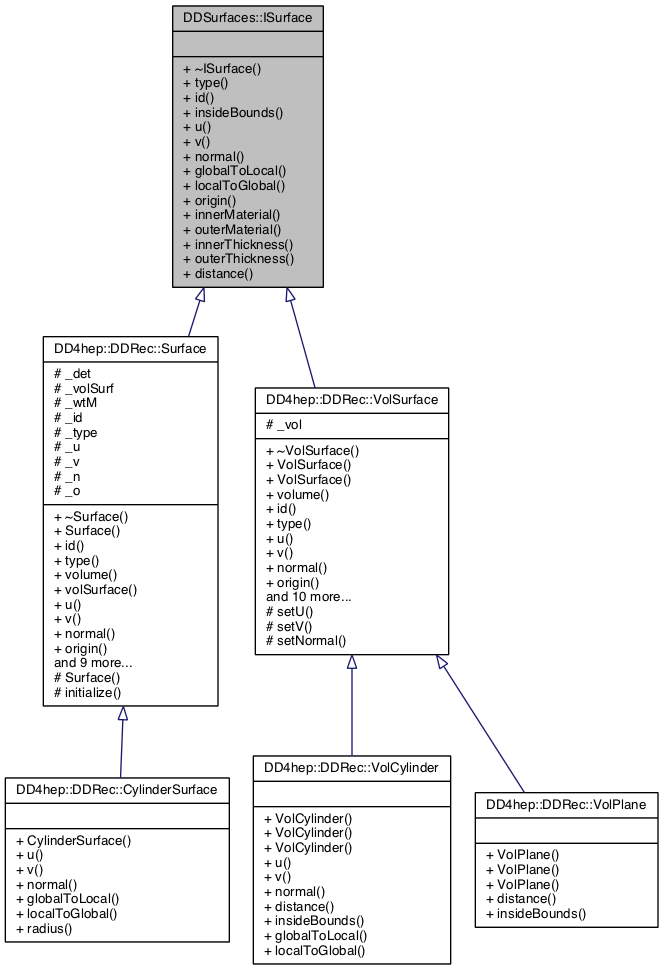
\includegraphics[height=180mm] {DDRec_surface_classes.png}
    \caption{Class diagram with the main classes describing detector
      surfaces and their relations.}
    \label{fig:ddrec_surfaces_classes}
  \end{center}
\end{figure}
\vspace{-0.1cm}

%=============================================================================
\subsection{namespace DDSurfacess}
\label{subsec:ddrec-ddsurfaces}
%=============================================================================



\newpage
%=============================================================================
\begin{thebibliography}{9}
\bibitem{bib:DD4hep} M. Frank et al, "DD4hep: A Detector Description Toolkit 
                for High Energy Physics Experiments",
                International Conference on Computing in High Energy and Nuclear Physics  
                (CHEP 2013), \\
                Amsterdam, Netherlands, 2013, proceedings.

\bibitem{bib:ROOT-tgeo} R.Brun, A.Gheata, M.Gheata, "The ROOT geometry package",\\
                    Nuclear Instruments and Methods {\bf{A}} 502 (2003) 676-680.
\bibitem{bib:geant4}  S. Agostinelli et al., 
                   "Geant4 - A Simulation Toolkit", \\
                    Nuclear Instruments and Methods {\bf{A}} 506 (2003) 250-303.

\end{thebibliography}
%=============================================================================
\end{document}
